\chapter{Marktmechanismus und Modellierung des Speicherbetriebs}
\label{ch:design_model}
\label{ch:requirements}

Das Engpassmanagement wird um eine Systemdienstleistung ergänzt, deren Gegenstand nicht die Leistungsanpassung selbst ist, sondern die Bereitschaft dazu im Fehlerfall.
Die Bemessung des finanziellen Ausgleichs aus dem Redispatch ist auf diese Bereitschaft nicht anwendbar, weil sie an die durchgeführte Anpassung anknüpft, wie in Abschnitt~\ref{sec:interim_conclusion} dargestellt.
Die Vergütung der Bereitschaft ist deshalb neu zu untersuchen, und dafür eignet sich ein kurativer Marktmechanismus, weil sich der kurative Reservierungspreis gegen die Erlöse der übrigen Vermarktung messen lässt.
In diesem Kapitel werden die Anforderungen an einen solchen Mechanismus abgeleitet, die kurative Reservierung als Produkt entworfen und der kurative Reservierungspreis mit einem Optimierungsmodell aus der Sicht des Anlagenbetreibers bestimmt.
Zum Abschluss wird der Referenzerlös des Modells gegen einen veröffentlichten Revenue-Index für \ac{BESS} auf Plausibilität geprüft.

\section{Anforderungen und Produkt}
\label{sec:market_requirements}

Aus den Befunden des Kapitels~\ref{ch:state_of_the_art} folgen Anforderungen, aus denen die kurative Reservierung als Produkt entwickelt wird.
Der folgende Katalog überführt die Befunde in Bedingungen, die sich an einem Mechanismus prüfen lassen, und gilt für die Umsetzung einer kurativen Systemführung, deren Vorhaltung marktlich beschafft wird.

\subsection{Anforderungskatalog}
\label{sec:requirements_catalogue}

\begin{description}
    \item[A1 -- Reaktionszeit] Die kurative Reservierung muss nach der Reaktionszeit differenziert sein, weil das betroffene Betriebsmittel die Reaktionszeit vorgibt und der Akteur sie nicht wählen kann.
    Der \ac{ÜNB} legt die zulässige Vorauslastung vor dem Fehlerfall fest und muss die Reaktionszeit der zugesagten Maßnahme dafür bereits kennen.
    Die zugesagte Reaktionszeit muss die Anlage deshalb bei jedem Abruf gleichbleibend erbringen, denn der \ac{ÜNB} plant die Vorauslastung im Vertrauen auf sie.
    \item[A2 -- Verbindlichkeit] Die Zusage muss binden und damit bei Nichterfüllung wirksame Sanktionen enthalten.
    Die Sanktion ist nötig, denn eine Nichterfüllung liegt bereits bei einer verspäteten Leistungsänderung vor.
    Aus einer verspäteten Leistungsänderung können Schäden am Betriebsmittel entstehen, die die Vergütung der Vorhaltung übersteigen.
    Die Sanktion darf deshalb nicht auf die entgangene Vergütung beschränkt bleiben.
    Eine Bemessung nach dem Grad der Abweichung scheidet aus, denn eine Leistungsänderung nach dem Ende des Überlastintervalls hat nicht einen verminderten, sondern gar keinen Wert.
    \item[A3 -- Lokationalität] Die Beschaffung muss netzknotenscharf erfolgen, denn dieselbe Leistungsänderung entlastet ein Betriebsmittel je nach Netzknoten unterschiedlich stark.
    Die Wirkung je Knoten muss der \ac{ÜNB} in seinen Vorschau- und Netzsicherheitsrechnungen mitprüfen.
    \item[A4 -- Bemessungsgegenstand] Die Vergütung muss an der vorgehaltenen Leistung und an der Bindungsdauer ansetzen, denn die kurative Bindung schränkt den Betrieb über ihre gesamte Dauer ein und nicht allein im Fehlerfall.
    Die Kosten fallen deshalb auch ohne Abruf an.
    Gegenstand der Vergütung ist die reservierte Leistung, ein Abruf wird daneben gesondert vergütet.
    Maßgeblich ist, dass die Leistungsänderung im Abruf erbracht werden kann.
    Die Erbringung fällt den Technologien unterschiedlich schwer, je nachdem, ob die Leistungsänderung einen bestimmten Betriebspunkt oder einen Energievorrat voraussetzt.
    \item[A5 -- Diskriminierungsfreiheit] Die Binnenmarktverordnung verlangt einen diskriminierungsfreien Zugang aller Technologien, wie in Abschnitt~\ref{sec:legal_framework} dargestellt, und der kurative Marktmechanismus setzt deshalb an den geforderten Eigenschaften an und nicht an der Technologie.
    In der Präqualifikation heißt das, technische und physikalische Eigenschaften zu prüfen und nicht die Art der Anlage.
    Der offene Zugang ist zugleich die Voraussetzung dafür, dass der \ac{ÜNB} am betroffenen Knoten unter mehreren Geboten das günstigste annehmen kann.
    Die Liquidität am Knoten folgt aus der Zahl der zugelassenen Anbieter und begrenzt, wie günstig das Gebot ausfällt.
    \item[A6 -- Teilnahme] Der kurative Marktmechanismus muss die Teilnahme für den Betreiber lohnend ausgestalten, weil der Betreiber über sein Gebot allein entscheidet und die Maßnahme ohne Gebot nicht verfügbar ist.
    Die marktliche Beschaffung ist damit nicht allein eine Frage der Zugangsform, sondern die Bedingung dafür, dass sich eine kurative Systemführung umsetzen lässt.
    \item[A7 -- Verträglichkeit] Der kurative Marktmechanismus muss neben den bestehenden Märkten bestehen können, ohne einen von ihnen zu verdrängen.
    Die kurative Reservierung greift auf dieselbe Leistung und denselben Ladezustand zu, die eine Anlage auch für die Regelleistung und für die Spotmärkte einsetzt.
    Ein kurativer Markt, der diese Ressourcen dauerhaft bindet oder höher vergütet als ein bestehender Markt mit gleichem Produktschnitt, zöge dessen Anbieter ab und ließe eine Systemdienstleistung ohne Teilnehmer zurück.
    Die Teilnahme ist deshalb so auszugestalten, dass die Anlage für die übrigen Märkte und für den Redispatch verfügbar bleibt.
    \item[A8 -- Umsetzbarkeit] Der kurative Marktmechanismus muss in die Betriebsprozesse integrierbar sein, die der \ac{ÜNB} für das Engpassmanagement bereits führt, nämlich in die Betriebsplanung, die Scharfschaltung und den Abruf.
    Die bezuschlagten Gebote müssen sich dafür zu einem kurativen Maßnahmenset zusammenfassen lassen, das der \ac{ÜNB} wie eine eigene kurative Maßnahme einplant und scharfschaltet.
\end{description}

\label{sec:market_design_comparison}

\label{sec:product_design}

\subsection{Die kurative Reservierung}
\label{sec:product_scope}
\label{sec:product_parameters}

Mit einer kurativen Reservierung sagt der Akteur dem \ac{ÜNB} eine Leistungsänderung für den Fehlerfall zu und geht dafür die kurative Bindung ein, nämlich ein Leistungsband und ein Ladezustandsband, innerhalb dessen die Anlage bleibt.
Der \ac{ÜNB} nimmt die Zusage in seine Einsatzplanung auf und ruft sie im Fehlerfall ab.
Die kurative Bindung besteht über die Bindungsdauer durchgehend, ein Abruf erfolgt nur im Fehlerfall.
Vergütet wird die Vorhaltung über den kurativen Reservierungspreis.
Ein Abruf wird gesondert vergütet.

Der Akteur nimmt die kurativ gebundene Leistung aus seiner übrigen Vermarktung heraus.
Daraus entstehen die Opportunitätskosten, die der Akteur über den kurativen Reservierungspreis ersetzt verlangt.
Eine Anlage kann beide Richtungen anbieten, aber jede Richtung bindet einen anderen Teil des Ladezustandsbandes und ist deshalb ein eigenes Gebot.
Gesperrt ist damit allein die zugesagte Leistung, während für das gebundene Zeitfenster kein allgemeines Handelsverbot gilt.
Neben Richtung und Leistung nennt ein Gebot die Reaktionszeitklasse, für die der Akteur einsteht.
Weil zu jeder Höhe der Überlast eine zulässige Dauer gehört, schaltet jede Reaktionszeit ein anderes Maß an Höherauslastung frei.
Die kurative Reservierung übernimmt deshalb die drei Klassen aus InnoSys~2030, nämlich unter zehn Sekunden, etwa zwei Minuten und bis 15 Minuten, wie in Abschnitt~\ref{sec:curative_functionality} beschrieben.
Wer die kürzeste Klasse erfüllt, erfüllt damit auch die längeren, sodass ein schneller Akteur in jeder Klasse anbieten kann.
Die Klassen ersparen dem \ac{ÜNB} die Rechnung mit der Reaktionszeit jeder einzelnen Anlage, und drei Stufen halten den Zugang zugleich für viele Technologien offen.
Die Bindungsdauer beträgt eine Zeitscheibe, also eine Stunde des Liefertages.

Den Abruf löst der \ac{ÜNB} aus, sobald nach einem Ausfall die Überlastung tatsächlich eintritt.
Der Akteur erhält zum Abruf ein Signal, auf das seine Anlage innerhalb der zugesagten Klasse reagiert.
Die Anlage hält die Leistungsänderung höchstens eine Stunde, und diese Stunde kann über zwei Zeitscheiben reichen.
Angenommen ist der ungünstigste Fall eines einstündigen Abrufs.
Bei einem Speicher hält das Ladezustandsband deshalb je zugesagtem Megawatt eine Megawattstunde vor, in positiver Richtung als gespeicherte Energie und in negativer Richtung als freien Speicherraum.
Andere Technologien wie Wind- und Photovoltaikanlagen müssen ebenso über die Bindungsdauer sicherstellen, dass sie ihre Einspeisung gegenüber dem gemeldeten Fahrplan um die zugesagte Leistung absenken können.
Die zugesagte Leistung einer solchen Anlage lässt sich dabei ähnlich wie die gesicherte Leistung bewerten, also als der Anteil der installierten Leistung, der über die Bindungsdauer mit hoher Wahrscheinlichkeit verfügbar ist.
Kraftwerke halten das Leistungsband entsprechend in ihrer Fahrplanbildung frei, was für sie weniger kritisch ist, weil ihre Einspeisung nicht von einer Wind- oder Solarprognose abhängt.
Der Abruf endet früher, sobald der \ac{ÜNB} den Engpass mit anderen Mitteln behoben hat.
Nach einem Abruf ist der Akteur für den restlichen Liefertag von der Vorhaltung freigestellt.
An die Stelle der Lieferpflicht tritt jedoch eine Nachlaufpflicht, nach der der Akteur seine Leistung nicht um die zugesagte Leistung in die den Engpass verschärfende Richtung zurückverschieben darf.
Wie lange die Nachlaufpflicht gilt, folgt aus dem Betrieb und bleibt hier offen.
Die gesonderte Vergütung des Abrufs umfasst die gelieferte Energie und die Nachlaufpflicht je Megawatt.
Die Höhe der Abrufvergütung ist eigens zu betrachten und bleibt hier außer Betracht.
Die bilanzielle Verantwortung für die Abweichung vom Fahrplan im Abruf liegt nicht beim Akteur, sondern beim \ac{ÜNB}, der den Abruf ausgelöst hat.

Die kurative Zusage führt der Akteur in den Planungsdaten mit, die er dem \ac{ÜNB} übermittelt.
Der Akteur weist zweierlei nach, nämlich dass seine Anlage die kurative Bindung über die Bindungsdauer eingehalten und im Abruf die Leistungsänderung innerhalb der Klasse erbracht hat.
Eine verspätete oder zu geringe Leistungsänderung bringt das Betriebsmittel nicht mehr in einen dauerbelastbaren Zustand, weshalb die Erfüllung binär ist.
Die Pönale knüpft deshalb nicht erst an einen gescheiterten Abruf, sondern schon an die fehlende Handlungsfähigkeit, weil die Vorauslastung auf der Zusage beruht.
Von der Pönale befreit den Akteur allein der Nachweis, dass seine Handlungsfähigkeit an einem unvorhersehbaren Ereignis außerhalb seines Betriebs scheiterte.
Ein solches Ereignis hat der Akteur dem \ac{ÜNB} unverzüglich zu melden, damit der \ac{ÜNB} Gegenmaßnahmen einleiten kann.
Die Sanktion kann von einer Strafzahlung über den Entzug der Präqualifikation bis zur Übernahme der entstandenen Schäden reichen.
Höhe und Form der Sanktion bestimmt die Untersuchung nicht, weil das Modell die daraus folgende Risikoprämie nicht trägt.

Ob ein Akteur die zugesagte Klasse erfüllen kann, prüft der \ac{ÜNB} vor dem ersten Gebot in der Präqualifikation, in der der Akteur die geforderte Reaktionszeit, die vorhaltbare Leistung und die Einhaltung des Ladezustandsbandes nachweist.
Die Reaktionszeit, die Leistung und das Ladezustandsband prüft die Präqualifikation der Regelleistung bereits, nämlich als Folgen eines Sollwerts des \ac{ÜNB}, als Leistung und als Arbeitsvermögen \cite{ubertragungsnetzbetreiber_deutschland_praqualifikationsverfahren_2024}.
Eine für die Regelleistung präqualifizierte Anlage weist die dort geprüften Eigenschaften nicht erneut nach, sodass sich ihr Aufwand auf die zusätzlichen Anforderungen der kurativen Zusage beschränkt.
Die Klasse bis 15 Minuten deckt die Präqualifikation der \ac{aFRR} und der \ac{mFRR} ab, während eine Anlage für die Klassen von etwa zwei Minuten und unter zehn Sekunden die schnellere Reaktion eigens nachweist.
Anlagen, die nicht an der Regelleistung teilnehmen, weisen alle drei Eigenschaften selbst nach.
Der Akteur gibt allein den Netzknoten seiner Anlage an, denn die Sensitivität des Standorts, also die Wirkung einer Leistungsänderung an diesem Knoten auf das Betriebsmittel, folgt aus dem Netzmodell des \ac{ÜNB}.
Wie in der Regelleistung bestätigt der Netzbetreiber, an dessen Netz die Anlage angeschlossen ist, dass Vorhaltung und Abruf an diesem Anschluss möglich sind.

Präqualifizierte Akteure bieten in einer gemeinsamen, täglichen Ausschreibung der deutschen \ac{ÜNB} für alle 24 Stunden des Folgetages, je Stunde und Richtung mit einem eigenen Gebotspreis in \EurMWh{}.
Die Zeitscheibe von einer Stunde entspricht der Dauer des ungünstigsten Abrufs.
Den Bedarf ermitteln die \ac{ÜNB} in den Rechenläufen ihrer Redispatchplanung am Vortag, sodass er vor dem Zuschlag feststeht.
Die Mindestgröße eines Gebots beträgt 25\,\si{MW}, die eine Anlage allein oder mehrere Anlagen am selben Netzknoten zusammen erreichen.
Anders als die Regelleistung, die Anlagen innerhalb einer Regelzone zusammenfasst, erlaubt die kurative Reservierung die Zusammenfassung nur je Netzknoten.
Maßgeblich für die Zusammenfassung ist allein die Wirkung am angegebenen Knoten.
Als Netzknoten sind zunächst allein die Knoten des 380-kV-Netzes relevant.
Der Kreis lässt sich später um die 110-kV-Knoten mit einem Direktkuppler zum 380-kV-Netz und danach um das gesamte 110-kV-Netz erweitern.

Einen Anspruch auf Zuschlag hat der Akteur nicht.
Die \ac{ÜNB} nehmen Gebote nach pay-as-bid, also zum jeweils gebotenen Preis, nur für die Zeitscheiben an, die sie benötigen.
Neben dem Gebotspreis nennt das Gebot eine Höchstleistung, von der die \ac{ÜNB} auch einen Teil bezuschlagen können.
Der bezuschlagte Teil darf die Mindestgröße nicht unterschreiten.
Für den Zuschlag vergleichen die \ac{ÜNB} jedes Gebot nach seiner Wirkung, also nach der Sensitivität des Netzknotens, mit dem präventiven Redispatch und den Maßnahmen in ihrem eigenen Verfügungsbereich.
Bezuschlagt wird kein einzelnes Gebot, sondern ein Verbund aus Geboten beider Richtungen, denn die Maßnahme muss sich bilanziell ausgleichen.
Im Verbund entlastet die eine Richtung an einem wirksamen Knoten den Engpass, während die Gegenrichtung an einem anderen Knoten den bilanziellen Ausgleich stellt.
Die \ac{ÜNB} geben die Zuschläge vor 23.30 Uhr des Vortages bekannt, damit der Akteur für die erste Stunde des Liefertages noch vor dem Handelsschluss zwischen den Regelzonen umplanen kann.
Weil der Zuschlag am Vortag feststeht und über die ganze Zeitscheibe bindet, heben Fahrplanänderungen nach der letzten Vorschaurechnung die Vorhaltung nicht mehr auf.

\section{Optimierung des Speicherbetriebs}
\label{sec:model_scope}

\label{sec:research_gap}
\label{sec:product_open_questions}
Für den \ac{ÜNB} bedeutet die kurative Reservierung vor allem neue Abläufe in der Systemführung, von der Ermittlung des Bedarfs über den Verbund der Gebote bis zum Nachweis der Erfüllung.
Ob sich eine systemweite Integration der kurativen Systemführung lohnt, hängt für den \ac{ÜNB} davon ab, ob der Nutzen die Kosten der Reservierung und ihrer Umsetzung übersteigt.
Welchen kurativen Reservierungspreis ein Akteur fordert, hängt davon ab, was ihm die Reservierung unter den bestehenden Nebenbedingungen an anderer Vermarktung nimmt.
Für die kurative Reservierung besteht kein Vergütungsrahmen, an dem sich ein Akteur ausrichten könnte.
Der kurative Reservierungspreis ist deshalb aus dem Betrieb des Speichers selbst zu bestimmen.
Der kurative Reservierungspreis wird dafür als der kleinste Preis bestimmt, bei dem ein \ac{BESS} eine Zeitscheibe voll reserviert, statt die Leistung anderweitig zu vermarkten.
Der kurative Reservierungspreis liefert die Kostenseite der Abwägung, der der \ac{ÜNB} den Nutzen gegenüberstellen kann.
Für die Bestimmung wird ein Optimierungsmodell aufgebaut, das abbildet, wie ein \ac{BESS} über einen Liefertag an mehreren Märkten zugleich vermarktet wird.
Für die kurative Reservierung gibt das Modell je Stunde und Richtung einen Preis in \EurMWh{} vor, im Folgenden vorgegebener Reservierungspreis genannt, auf den der Betreiber seine Vermarktung einstellt.
Abbildung~\ref{fig:modellkette} zeigt den Weg eines Liefertages von den Marktdaten über die Dispatch-Optimierung bis zu den Ergebnissen.

\begin{figure}[htbp]
    \centering
    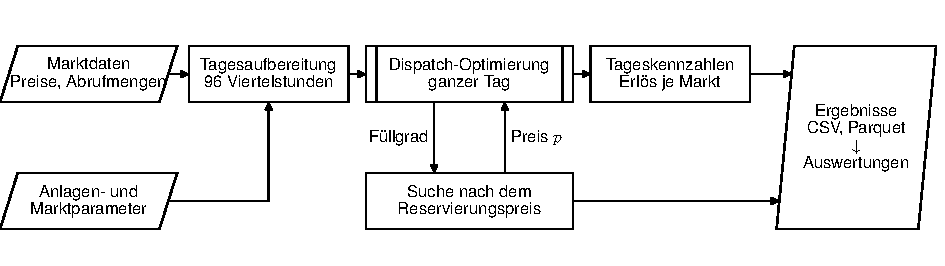
\includegraphics[width=\textwidth]{figures/chapter_3/modellkette.pdf}
    \caption{Modellkette eines Liefertages von den Marktdaten bis zu den Ergebnissen.}
    \label{fig:modellkette}
\end{figure}

Eingangsdaten sind die Marktdaten, nämlich die Preise und Abrufmengen des Jahres 2025, während die Anlagen- und Marktparameter im Modell festgelegt sind.
Die Tagesaufbereitung schneidet die Eingangsdaten je Liefertag in 96 Viertelstunden.
Die Dispatch-Optimierung maximiert den Erlös der Anlage über den ganzen Tag bei einem vorgegebenen Reservierungspreis je Stunde und Richtung.
Die Suche nach dem kurativen Reservierungspreis ist eine Schleife aus solchen Optimierungen: Sie setzt den vorgegebenen Reservierungspreis, liest die reservierte Leistung je Zeitscheibe zurück und ändert den vorgegebenen Reservierungspreis, bis je Zeitscheibe der kleinste Wert gefunden ist, bei dem die Anlage voll reserviert.
Ausgangsdaten sind alle Größen der Optimierung, nämlich der Erlös je Markt als wichtigste Tageskennzahl, die Verteilung der Leistung auf die Märkte, die Reservierung je Zeitscheibe und der Ladezustand.
Die Ausgangsdaten werden als CSV- und Parquet-Dateien abgelegt und daraus ausgewertet.

\subsection{Ansatz und Lösungsverfahren}
\label{sec:model_assumptions}

Das Modell führt als Bezug den Referenzfahrplan mit, also den Fahrplan ohne kurative Bindung aus einem Lauf ohne kurative Reservierung, koppelt den Ladezustand über den Tag und entscheidet alle Märkte gemeinsam.
Der Referenzfahrplan zeigt damit, was die Reservierung verdrängt.
Der Erlös des Referenzfahrplans ist der Referenzerlös.
Die Opportunitätskosten der Reservierung entstehen damit im Modell selbst, sodass kein gesonderter Kostenansatz für die Vorhaltung nötig ist.
Die Kopplung des Ladezustands bindet auch die Stunden vor einer Zeitscheibe, weil das Ladezustandsband die Energie oder den Speicherraum schon vorher bereithalten lässt.
Alle Märkte entscheidet das Modell gemeinsam und mit vollständiger Preiskenntnis, während der Akteur in Wirklichkeit nacheinander entscheidet, von der \ac{FCR} am Vortag bis zum regelzoneninternen Handel fünf Minuten vor Lieferbeginn.
Die Optimierung in einem Lauf mit vollständiger Preiskenntnis ist gewählt, weil eine Preisprognose dem Ergebnis eine weitere Annahme hinzufügte, deren Fehler sich vom Effekt der Reservierung nicht trennen ließe.
Der Abstand zum Betrieb eines Akteurs ist dabei bekannt und begrenzt, denn eine prognosegestützte Strategie erreicht im kontinuierlichen Intraday-Handel rund neunzig Prozent des unter vollständiger Preiskenntnis erzielbaren Erlöses \cite{hornek_value_2025}.
Der Erlös des Modells ist damit eine obere Schranke der übrigen Vermarktung.

Gelöst wird je Liefertag ein eigenes Problem, sodass kein Ladezustand in den Folgetag übergeht und die Tage untereinander vergleichbar bleiben.
Zielfunktion und Nebenbedingungen sind linear, sodass das Problem im Basisfall ein lineares Programm ist und die kurative Reservierung jeden Wert zwischen null und der Anschlussleistung annehmen darf.
Zur Untersuchung einzelner vorgegebener Reservierungspreise kann für die kurative Reservierung eine Mindestgröße festgelegt werden, in der Sensitivität 25\,\si{MW}.
Die Mindestgröße macht die Reservierung halbstetig und verlangt je Stunde und Richtung eine Binärvariable, sodass das Problem gemischt-ganzzahlig wird, wie in Abschnitt~\ref{sec:input_data} beschrieben.
Gelöst wird in beiden Fällen mit Gurobi 13.0.2, für das gemischt-ganzzahlige Programm mit einer relativen Optimalitätslücke von 0,01 Prozent und einem Zeitlimit von 60 Sekunden je Lauf als Abbruchkriterium \cite{gurobi_reference_2026}.

Das Modell betrachtet eine einzelne Anlage als Preisnehmer, denn gesucht ist der kurative Reservierungspreis aus der Sicht eines Betreibers.
Netzrestriktionen, die Zusammenfassung mehrerer Anlagen zu einem Pool und die Gegenseite der Maßnahme bildet das Modell nicht ab.
Ohne Netzmodell ist der kurative Bedarf nicht räumlich aufgelöst, sodass jede Zeitscheibe gleich behandelt wird.
Die Abrufwahrscheinlichkeit bleibt außer Betracht, und der Zuschlag in den Regelleistungsmärkten gilt zu den berücksichtigten Preisen als sicher.
Beide Vereinfachungen sind mit dem Produkt vereinbar: Weil ein Abruf gesondert vergütet wird, fließt er nicht in den kurativen Reservierungspreis ein, und die sicheren Zuschläge lösen die Erlöse am Regelleistungsmarkt vom Bietverhalten.
Nicht Teil des Modells sind die gesonderte Vergütung eines Abrufs, nämlich der gelieferten Energie und der Nachlaufpflicht, und die Pönale mit der Risikoprämie, die aus ihr folgt.
Der ermittelte kurative Reservierungspreis ist damit der opportunitätskostenbasierte Teil des Gebots und nicht das Gebot.
Die Rückwirkung der Speicher auf die Preise bleibt ebenfalls außer Betracht, sodass die Preise des Jahres 2025 als gegeben gelten.
Ein Zubau im Gigawattmaßstab drängt die zusätzliche Leistung überwiegend in die Arbitrage, weil die Regelleistungsmärkte mengenmäßig begrenzt sind \cite{garttan_battery_2025}.
Dort verzehren Speicher die Spreads, indem sie Niedrigpreisphasen anheben und Hochpreisphasen absenken \cite{rystad_energy_renewables__power_analytics_energy_2026}.
Der Szenariorahmen 2030 ordnet die Untersuchung qualitativ ein und geht nicht als Eingangsgröße in das Modell.

\label{sec:storage_modelling}

\label{sec:valuation_task}

\label{sec:lp_gurobi}

\subsection{Anlage, Speicher und Zielfunktion}
\label{sec:objective_variables}
\label{sec:storage_model}

Innerhalb dieser Grenzen wird eine einzelne Anlage abgebildet.
Die Anlage ist ein \ac{BESS} mit 100\,\si{MW} je Richtung und 250\,\si{MWh} Speicherkapazität, also einem Energieinhalt je Leistung von 2,5 Stunden.
Die Auslegung liegt über dem Bereich von ein bis zwei Stunden, den die Großspeicher in Betrieb erreichen, und im Bereich der geplanten Anlagen, wie in Abschnitt~\ref{sec:actor_comparison} dargestellt.
Laden und Entladen laufen mit einem Wirkungsgrad von 0,95 je Richtung, woraus ein Umlaufwirkungsgrad von 0,9025 folgt.
Der nutzbare Ladezustand liegt zwischen 5 und 95 Prozent, sodass die Anlage 225\,\si{MWh} bewegen kann.
Bei voller Anschlussleistung reicht dieser nutzbare Ladezustand für gut zwei Stunden Lieferung.
Jede Reservierung nimmt ihr Ladezustandsband aus dem nutzbaren Ladezustand.
Die Degradation belastet mit 8 Euro je Megawattstunde Durchsatz den Handel und die gelieferte Arbeit, nicht aber die Vorhaltungen.
Der Satz entspricht der Größenordnung, die sich aus den Investitionskosten eines schlüsselfertigen Speichersystems und seinem Lebensdauerdurchsatz ergibt \cite{rystad_energy_renewables__power_analytics_energy_2026}.
Der Verschleiß hängt tatsächlich von Temperatur, Ladezustand und Strom ab und ließe sich erst mit zusätzlichen Binärvariablen abbilden \cite{kumtepeli_energy_2020}.
Das Modell nimmt die Vereinfachung in Kauf, weil die Preissuche das Tagesmodell einige hundert Mal je Tag löst.
Der Liefertag zerfällt in 96 Viertelstunden, und die Blockprodukte binden Zeitscheiben von einer und von vier Stunden.
Entscheidungsvariablen sind die Leistungen an den Energiemärkten, die vorgehaltenen Leistungen der Regelleistung, die kurativ reservierte Leistung je Richtung, die gelieferte \ac{aFRR}-Arbeit mit ihrem Ausgleich am \ac{IDC} und der Ladezustand, alle stetig und nichtnegativ.
Anhang~\ref{anh:modell} führt die Variablen vollständig auf.
Die Zielfunktion maximiert den Nettoerlös eines Liefertages über alle geführten Märkte abzüglich der Degradationskosten.
\begin{equation}
    \label{eq:zielfunktion}
    \max \; E^{\mathrm{BESS,ges}} = E^{\mathrm{DA}} + E^{\mathrm{IDC}} + E^{\mathrm{FCR}} + E^{\mathrm{aFRR,L}} + E^{\mathrm{aFRR,E}} + E^{\mathrm{kur}} \; - \; K^{\mathrm{deg}}
\end{equation}
Die vollständige Formulierung mit allen Nebenbedingungen steht in Anhang~\ref{anh:modell}.

Die Ladezustandsbilanz führt den Speicherinhalt über den Tag fort, wobei allein der Handel und die gelieferte \ac{aFRR}-Arbeit ihn bewegen und die Wirkungsgrade beider Richtungen eingehen.
Anfang und Ende eines Tages tragen denselben Ladezustand, damit kein Tag mit eingelagerter Energie endet und die Tage untereinander vergleichbar bleiben.
Der gemeinsame Wert ist im Basisfall auf 50 Prozent der Speicherkapazität gesetzt, alternativ wählt das Modell den Anfangszustand frei, und der Endzustand folgt ihm.
Auf jeder Seite teilen sich der Handel, die \ac{aFRR}, die kurative Reservierung und die auf beiden Seiten stehende \ac{FCR} die Anschlussleistung.
Eine kurativ reservierte Leistung steht deshalb keinem anderen Markt zur Verfügung.

\subsection{Abbildung der Märkte}
\label{sec:input_data}
\label{sec:constraints}

Das Modell führt neben der kurativen Reservierung die Märkte, an denen ein \ac{BESS} heute seine Erlöse erzielt, nämlich den \ac{DA}, den \ac{IDC}, die \ac{FCR} und die \ac{aFRR} mit Leistung und Arbeit.
Nicht geführt werden die Intraday-Auktionen, weil das Optimierungsmodell den Fahrplan sonst zu jeder weiteren Handelsgelegenheit neu bewerten müsste, und die \ac{mFRR}, wie in Abschnitt~\ref{sec:balancing_procurement} begründet.
Der Ausschluss der Intraday-Auktionen ist damit eine Vereinfachung des Optimierungsmodells.
\ac{DA}, \ac{IDC} und \ac{aFRR}-Arbeit bewegen den Ladezustand, während \ac{FCR}, \ac{aFRR}-Leistung und die kurative Reservierung Leistung und ein Ladezustandsband binden, ohne Energie umzuschlagen.
Jeder Markt trägt seinen eigenen Produktzuschnitt, seinen Energievorhalt und seinen Preis.

Auswertungszeitraum ist das Jahr 2025.
Weil der \ac{DA} erst seit dem 01.10.2025 in Viertelstunden gehandelt wird, gilt davor sein Stundenpreis für alle vier Viertelstunden \cite{ffe_saegezahn_2026}.
Die beiden Tage der Zeitumstellung führt das Modell mit 96 Viertelstunden, indem es die fehlende Stunde im Frühjahr durch Platzhalter ersetzt, im Herbst die zweite Ausführung der doppelten Stunde verwirft und die betroffene Stunde in beiden Fällen sperrt.

\subsubsection*{Day-Ahead}
Die Preisreihe des \ac{DA} ist der Auktionspreis der Gebotszone Deutschland und Luxemburg, bezogen aus den Energy-Charts des Fraunhofer ISE \cite{energy_charts_strompreise_2026}.
Die Käufe und Verkäufe am \ac{DA} gleichen sich über den Tag energetisch aus und müssen ihre eigenen Degradationskosten decken.
So bildet das Modell nach, dass der Betreiber am \ac{DA} bietet, bevor der Zuschlag der kurativen Reservierung feststeht, und die Reservierung den Handel dort nicht mitfinanziert.
Ein Geschäftspaar am \ac{DA} kommt deshalb nur zustande, wenn die Preisspanne der Arbitrage die Degradationskosten in der Summe des Tages übersteigt.
Der Erlös am \ac{DA} ist die über den Tag summierte Differenz aus Verkauf und Kauf, jeweils zum Auktionspreis der Viertelstunde.

\begin{equation}
    \label{eq:erloes_da}
    E^{\mathrm{DA}} = \Delta t \sum_{t \in \mathcal{T}} p^{\mathrm{DA}}_t \left( P^{\mathrm{DA,aus}}_t - P^{\mathrm{DA,ein}}_t \right)
\end{equation}

\subsubsection*{Kontinuierlicher Intraday-Handel}
Auch am \ac{IDC} handelt die Anlage Energie, bewertet wird dieser Handel aber je Viertelstunde mit dem \ac{ID1}, dem Preisindex der letzten Stunde vor Lieferbeginn, ebenfalls aus den Energy-Charts \cite{energy_charts_strompreise_2026}.
Im kontinuierlichen Handel kommt jedes Geschäft zu seinem eigenen Preis zustande, sodass es für eine Viertelstunde keinen einheitlichen Preis gibt.
Eine viertelstundenübergreifende Arbitrage greift deshalb auf volumengewichtete Durchschnittspreise zurück.
Das Modell lässt nur Arbitrage zwischen Viertelstunden zu, während ein Betreiber dieselbe Viertelstunde mehrfach handeln und eine frühere Position innerhalb desselben Lieferzeitpunktes wieder glattstellen kann.
Was der Betreiber damit zusätzlich verdient, ließe sich nur aus den Orderbüchern ablesen.
Ohne Orderbücher bleibt ein rollierender Handel mit laufender Neubewertung eine Schätzung.
Weil ein Betreiber dieselbe Viertelstunde mehrfach handeln kann, verbessert jede zusätzliche Handelsmöglichkeit den erzielbaren Preis, sodass der \ac{IDC} insgesamt mehr trägt als ein einzelnes Geschäft zum Index.
Das Modell bildet den Vorteil des mehrfachen Handels über einen Aufschlag ab, der Verkäufe über und Käufe unter dem Index bewertet und den Spread damit weitet.
Die Höhe des Aufschlags wird als Sensitivität variiert.
Der Höchst- und der Niedrigstpreis einer Viertelstunde wären ein anderes Maß für den Vorteil des mehrfachen Handels, bleiben aber außer Betracht, weil sie keine Menge führen und damit offen bliebe, wie viel Leistung zu ihnen handelbar gewesen wäre.
Der Erlös am \ac{IDC} ist die über den Tag summierte Differenz aus Verkäufen zum um den halben Aufschlag $a$ erhöhten und Käufen zum um den halben Aufschlag gesenkten \ac{ID1}.

\begin{equation}
    \label{eq:erloes_idc}
    E^{\mathrm{IDC}} = \Delta t \sum_{t \in \mathcal{T}} p^{\mathrm{ID1}}_t \left[ \left( 1 + \frac{a}{2} \right) P^{\mathrm{IDC,aus}}_t - \left( 1 - \frac{a}{2} \right) P^{\mathrm{IDC,ein}}_t \right]
\end{equation}

\subsubsection*{\acs{FCR}}
Die \ac{FCR} wird zu einem Einheitspreis bezuschlagt, und das Modell übernimmt diesen Preis je Vier-Stunden-Zeitscheibe in \EurMWh{} aus den Ausschreibungsergebnissen auf regelleistung.net \cite{regelleistung_ausschreibungsdaten_2026}.
Weil die \ac{FCR} allein die Bereitschaft vergütet und keinen Arbeitspreis kennt, ist ihr Erlös der Leistungspreis mal der vorgehaltenen Leistung.
Je vorgehaltenem Megawatt bindet die \ac{FCR} ein Ladezustandsband von einer Viertelstunde, das für den Handel nicht mehr zur Verfügung steht.
Die \ac{FCR} ist symmetrisch und bleibt über ihre Zeitscheibe von vier Stunden konstant.
In Gleichung~\ref{eq:erloes_fcr} bezeichnet $s(t)$ die Vier-Stunden-Zeitscheibe, in der die Viertelstunde $t$ liegt.

\begin{equation}
    \label{eq:erloes_fcr}
    E^{\mathrm{FCR}} = \Delta t \sum_{t \in \mathcal{T}} p^{\mathrm{FCR}}_{s(t)} \, P^{\mathrm{FCR}}_{s(t)}
\end{equation}

\subsubsection*{\acs{aFRR}-Leistung}
Anders als die \ac{FCR} wird die \ac{aFRR}-Leistung nach pay-as-bid vergütet, weshalb das Modell den mengengewichteten Durchschnitt der Zuschläge einer Vier-Stunden-Zeitscheibe aus den Ausschreibungsergebnissen auf regelleistung.net ansetzt \cite{regelleistung_ausschreibungsdaten_2026}.
Den höchsten Zuschlag setzt das Modell nicht an, weil ein Anbieter ihn nicht sicher erreicht.
Die Merit-Order der Ausschreibung, also die nach ihrem Preis geordneten Gebote, zeigt, welches Volumen zu welchem Preis bezuschlagt wird.
Der mengengewichtete Durchschnitt der Merit-Order trifft den Wert, den ein Anbieter im Mittel erzielt.
Im Jahr 2025 lag der höchste Zuschlag nach eigener Auswertung der Ausschreibungsdaten im Median 16 Prozent über dem Durchschnitt in der positiven und 22 Prozent in der negativen Richtung.
Ein höherer Zuschlag beruht nicht auf einem technischen Vorteil, denn alle bezuschlagten Gebote erbringen dieselbe Leistung, sondern auf dem Bietverhalten.
Der höchste Zuschlag wird deshalb allein als Sensitivität geführt.

Der Erlös der \ac{aFRR}-Leistung ist ihr Leistungspreis mal der vorgehaltenen Leistung.
Je vorgehaltenem Megawatt bindet sie ein Ladezustandsband von einer Stunde.
Vorgehalten wird je Richtung, und die Vorhaltung bleibt über die Vier-Stunden-Zeitscheibe konstant.
Für die \ac{aFRR}-Leistung führt das Modell drei Sensitivitäten, nämlich ohne \ac{aFRR}, mit dem mengengewichteten Mittelpreis und mit dem höchsten Zuschlag, und der Basisfall rechnet mit dem Mittelpreis.

\begin{equation}
    \label{eq:erloes_afrr_l}
    E^{\mathrm{aFRR,L}} = \Delta t \sum_{t \in \mathcal{T}} \sum_{r} p^{\mathrm{aFRR}}_{s(t),r} \, P^{\mathrm{aFRR}}_{s(t),r}
\end{equation}

\subsubsection*{\acs{aFRR}-Arbeit}
Die \ac{aFRR}-Arbeit vergütet der \ac{ÜNB} nach dem Grenzpreisverfahren, wie in Abschnitt~\ref{sec:balancing_procurement} beschrieben.
Die \ac{aFRR}-Arbeit bewertet das Modell je Viertelstunde und Richtung mit dem volumengewichteten Mittel der Grenzpreise der Plattform PICASSO, gebildet über die 225 Vier-Sekunden-Zyklen einer Viertelstunde aus der Transparenzplattform der ENTSO-E \cite{entsoe_transparency_2026}.
Als Gewicht dient in der Mittelung der Sollwert von netztransparenz.de, weil das je Zyklus aktivierte Volumen nicht veröffentlicht wird \cite{netztransparenz_regelenergie_2026}.
Viertelstunden ohne Abruf einer Richtung bleiben für diese Richtung gesperrt.
Die Anlage liefert \ac{aFRR}-Arbeit anteilig am deutschen Abruf, im Verhältnis ihrer vorgehaltenen Leistung zur ausgeschriebenen Menge, und wählt keine einzelnen Viertelstunden aus.
Wie viel Arbeit die Anlage liefern darf, prüft eine Sensitivität, die den anteiligen Abruf gegen eine freie Lieferung bis zur eigenen Reservierung und bis zu zehn Prozent des deutschen Abrufs stellt.
Die gelieferte Arbeit stammt aus dem Speicher und wird am \ac{IDC} erst in einer späteren Viertelstunde ausgeglichen und nie in derselben, denn der Abruf steht erst nach der Viertelstunde fest.
Der Ausgleich ist eine eigene Größe je Viertelstunde und Richtung, und seine Menge schließt sich über den Tag gegen die gelieferte Arbeit.
Der Erlös der \ac{aFRR}-Arbeit ist ihr Arbeitspreis mal der gelieferten Energie, vermindert beziehungsweise erhöht um den Wert des Ausgleichs in der Viertelstunde, in der er stattfindet.

\begin{equation}
    \label{eq:erloes_afrr_e}
    E^{\mathrm{aFRR,E}} = \Delta t \sum_{t \in \mathcal{T}} \left[ p^{\mathrm{aFRR,E}}_{t,\mathrm{pos}} P^{\mathrm{aFRR,E}}_{t,\mathrm{pos}} + p^{\mathrm{aFRR,E}}_{t,\mathrm{neg}} P^{\mathrm{aFRR,E}}_{t,\mathrm{neg}} - p^{\mathrm{ID1}}_t P^{\mathrm{aus}}_{t,\mathrm{pos}} + p^{\mathrm{ID1}}_t P^{\mathrm{aus}}_{t,\mathrm{neg}} \right]
\end{equation}

\subsubsection*{Kurative Reservierung}
Die Zielfunktion trägt für die kurative Reservierung den Erlös aus vorgegebenem Reservierungspreis mal reservierter Leistung.
Die Anlage reserviert deshalb nur dann, wenn der vorgegebene Reservierungspreis den Wert der Handelsaktionen übersteigt, die die Reservierung in derselben Stunde an den übrigen Märkten verdrängt.
Die reservierte Leistung ist eine Variable je Richtung mit vorgegebenem Reservierungspreis, die über eine Zeitscheibe von einer vollen Stunde zur nächsten konstant bleibt, also für vier aufeinanderfolgende Viertelstunden.
Die Reservierung tritt in dieselbe Leistungsschranke wie die \ac{FCR} und die \ac{aFRR} und bindet darüber hinaus ein Ladezustandsband, das den Abruf über die Bindungsdauer deckt.
Die positive und die negative Reservierung betrachtet das Modell getrennt, jede mit eigener Leistung und eigenem Ladezustandsband.
\begin{equation}
    \label{eq:erloes_kur}
    E^{\mathrm{kur}} = \Delta t \sum_{t \in \mathcal{T}} \sum_{r} \pi_{s(t),r} \, P^{\mathrm{kur}}_{s(t),r}
\end{equation}
Die Mindestgröße von 25\,\si{MW} ist ein Parameter des Produkts, sodass eine Stunde entweder ungebunden bleibt oder mit mindestens diesem Wert reserviert wird.
Im Basisfall rechnet das Modell mit stetiger Reservierung, weil jeder Tag viele Läufe verlangt.
Die Mindestgröße wird als Sensitivität zugeschaltet, um ihre Wirkung zu prüfen.

\label{sec:model_scope_verification}

\subsection{Bestimmung des kurativen Reservierungspreises}
\label{sec:reservation_price_search}
\label{sec:weber_exclusion}

Den kurativen Reservierungspreis bestimmt eine Suche außerhalb der Optimierung, die das Tagesmodell wiederholt aufruft und aus jedem Lauf die reservierte Leistung abliest.
Der Füllgrad einer Stunde und Richtung ist der Anteil der reservierten an der höchstmöglichen Leistung.
Als voll reserviert gilt eine Stunde, wenn höchstens ein Hundertstel Prozent der Anschlussleistung fehlt, also 0,01\,\si{MW} von 100\,\si{MW}.
Die Toleranz ist nötig, weil der Solver die Nebenbedingungen nur bis auf seine Zulässigkeitstoleranz von $10^{-6}$ einhält, und sie liegt mit 0,01\,\si{MW} über dem numerischen Rauschen.
Gesucht ist je Stunde und Richtung der kleinste vorgegebene Reservierungspreis, bei dem die Stunde voll reserviert ist.
Die Suche läuft in zwei gleich aufgebauten Iterationen, wie Abbildung~\ref{fig:reservierungspreis_ablauf} zeigt und Anhang~\ref{anh:ablauf} mit allen Schritten darstellt.
% VERSCHOBEN 18.09.2026, Kommentar des Verfassers: Der Satz stand hier auf
% Seite 42, waehrend die Bisektion erst nach den beiden Abbildungen auf Seite 43
% erklaert wird. Er eroeffnet jetzt den Absatz zur Bisektion.
%Jede Iteration bestimmt zuerst die Grenzen eines Suchintervalls und halbiert dieses Intervall danach für jede Stunde in derselben Bisektion.

\begin{figure}[H]
    \centering
    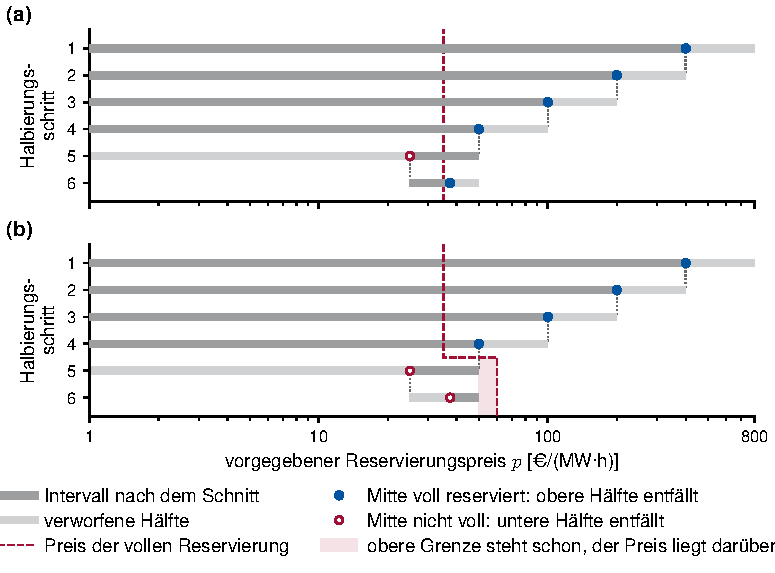
\includegraphics[width=\textwidth]{figures/chapter_3/reservierungspreis_bisektion.pdf}
    \caption{Bisektion für eine Beispielstunde, (a) bei festem Preis der vollen Reservierung, (b) wenn dieser Preis während der Suche steigt und die obere Grenze ihm nicht mehr folgt. Die Preisachse ist logarithmisch, geprüft wird stets die Mitte des Intervalls.}
    \label{fig:reservierungspreis_bisektion}
\end{figure}

\begin{figure}[t]
    \centering
    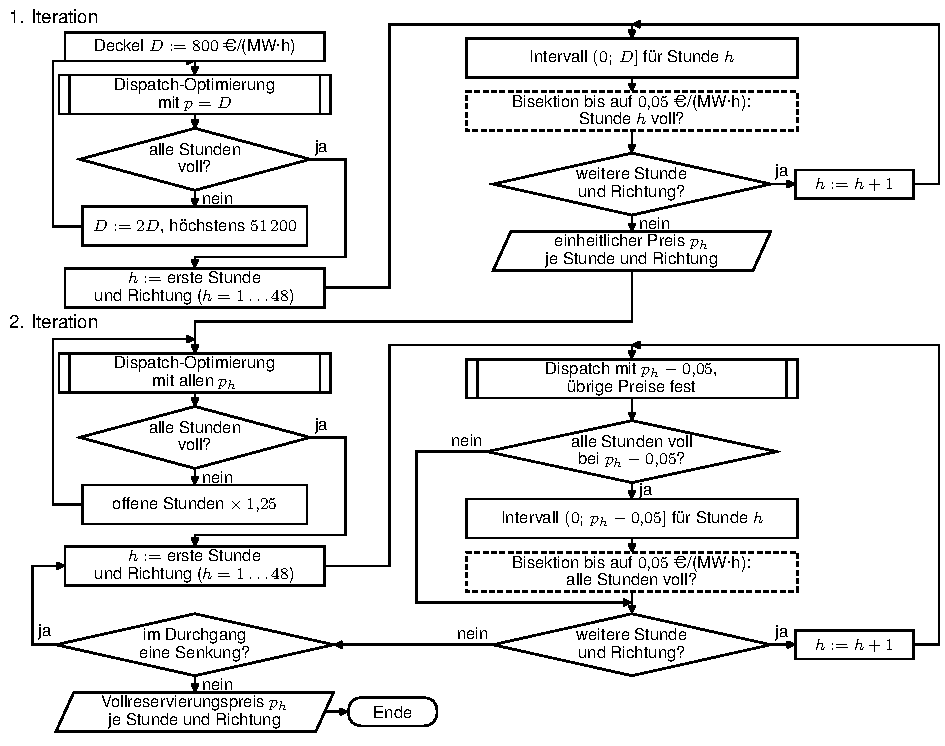
\includegraphics[width=\textwidth]{figures/chapter_3/reservierungspreis_ablauf_kompakt.pdf}
    \caption{Bestimmung des kurativen Reservierungspreises in zwei Iterationen, Symbole nach DIN 66001. Der gestrichelte Kasten fasst die Bisektion zusammen, die Anhang~\ref{anh:ablauf} ausführlich zeigt.}
    \label{fig:reservierungspreis_ablauf}
\end{figure}

% HIERHER VERSCHOBEN 18.09.2026, Kommentar des Verfassers. Der Satz traegt
% jetzt die These des Absatzes.
Jede Iteration bestimmt zuerst die Grenzen eines Suchintervalls und halbiert dieses Intervall danach für jede Stunde in derselben Bisektion.
% NEU 18.09.2026, Kommentar des Verfassers: einleiten, wie die Bisektion den
% Preis findet. Bis dahin war nicht gesagt, was die beiden Grenzen bedeuten und
% warum der gesuchte Preis zwischen ihnen liegt. Alte Fassung des Absatzanfangs:
%Die Bisektion prüft die Mitte des Intervalls mit einem Lauf.
Die untere Grenze des Suchintervalls reicht für die volle Reservierung nicht aus, während die obere Grenze dafür ausreicht.
Der gesuchte Preis liegt damit zwischen beiden Grenzen, und die Bisektion prüft die Mitte des Intervalls mit einem Lauf.
Reicht der Preis in der Mitte für die volle Reservierung, wird die Mitte zur oberen Grenze, sonst zur unteren.
Der Preis muss in der ersten Iteration die betrachtete Stunde voll reservieren, in der zweiten alle Stunden des Tages.
Die Bisektion endet, sobald das Intervall nicht breiter als 0,05\,\EurMWh{} ist.
Das Ergebnis ist die obere Grenze des letzten Intervalls, also der kleinste vorgegebene Reservierungspreis, der nachweislich für die volle Reservierung reicht.
Teil (a) von Abbildung~\ref{fig:reservierungspreis_bisektion} zeigt den Weg der Intervalle auf einer logarithmischen Preisachse.

Die erste Iteration gibt in jedem Lauf allen Stunden denselben Reservierungspreis vor.
Die obere Grenze der ersten Iteration ist ein Deckel von 800\,\EurMWh{}.
Der Deckel verdoppelt sich, bis alle Stunden voll reserviert sind, höchstens bis 51.200\,\EurMWh{}.
Bleibt eine Stunde auch beim höchsten Deckel nicht voll reserviert, gibt es für sie keinen Preis, denn dann verhindert eine Restriktion des Modells die Reservierung und nicht der Preis.
Das tritt allein an den beiden Tagen der Zeitumstellung ein, an denen eine Stunde gesperrt ist.
Nur dort steigt der Deckel bis 51.200\,\EurMWh{}, während er an allen übrigen Tagen bei 800\,\EurMWh{} bleibt.
Je Stunde halbiert die Bisektion dann das Intervall von null bis zum Deckel.
Bei einem Deckel von 800\,\EurMWh{} sind bis zu einer Breite von 0,05\,\EurMWh{} 14 Halbierungen nötig.
Würde jedes der 48 Paare aus Stunde und Richtung für sich halbiert, wären je Tag 48 mal 14, also 672 Läufe nötig.
Alle Paare mit derselben Intervallmitte teilen sich jedoch einen Lauf, weil das Tagesmodell alle Stunden bei einem einheitlichen vorgegebenen Reservierungspreis zugleich löst.
Darum genügen in den ausgewerteten Tagen 84 bis 167 Läufe je Tag, im Mittel rund 130.

Die erste Iteration allein reicht nicht aus, denn nach ihr können Stunden, deren obere Grenze schon feststeht, wieder für die Arbitrage genutzt werden.
Der Fehler liegt im Verfahren, denn der Preis, bei dem eine Stunde voll reserviert, hängt nicht von ihrem eigenen vorgegebenen Reservierungspreis allein ab, sondern von den vorgegebenen Reservierungspreisen aller 48 Stunden und Richtungen des Tages zusammen.
Die Zeitkopplung der kurativen Reservierung über den Ladezustand verschiebt den Lösungsraum, sobald der vorgegebene Reservierungspreis einer anderen Stunde steigt.
Die erste Iteration liefert deshalb je Stunde nur einen Startwert, gefunden unter einem für den ganzen Tag einheitlichen vorgegebenen Reservierungspreis.
Werden die Preise der ersten Iteration gemeinsam vorgegeben, bleiben in den ausgewerteten Tagen 18 Prozent der Stunden in positiver und 23 Prozent in negativer Richtung unter der vollen Reservierung.
Teil (b) von Abbildung~\ref{fig:reservierungspreis_bisektion} zeigt schematisch, was geschieht, sobald dieser Preis während der Suche steigt: Liegt er über der schon gesetzten oberen Grenze, ist jede weitere Mitte nicht voll, und die Bisektion hebt nach ihrer Regel nur die untere Grenze an, bis das Intervall sich schließt.
Die obere Grenze prüft die Bisektion nie erneut, sodass sie bei einem vorgegebenen Reservierungspreis endet, bei dem die Stunde nicht mehr voll ist, ohne es zu bemerken.
Einzelne Stunden nacheinander anzuheben führt ebenfalls nicht zum Ziel, weil eine gerade gefüllte Stunde wieder herausfällt, sobald die nächste Stunde steigt.

Die zweite Iteration gibt deshalb in jedem Lauf je Stunde und Richtung einen eigenen Reservierungspreis vor und startet mit den Preisen der ersten Iteration.
Solange eine Stunde nicht voll reserviert ist, hebt die zweite Iteration alle offenen Stunden zugleich um ein Viertel an.
Die so erreichten Preise reichen für die volle Reservierung, können wegen der groben Schritte aber zu hoch sein.
Stunde für Stunde prüft die zweite Iteration deshalb mit einem Lauf, ob alle Stunden bei einem um 0,05\,\EurMWh{} niedrigeren Preis dieser Stunde voll reserviert bleiben.
Bleiben alle Stunden voll, sucht die Bisektion zwischen null und dem gesenkten Preis den kleinsten noch ausreichenden Preis der Stunde.
Die übrigen Stunden behalten in den Läufen der Bisektion ihren Preis.
Die zweite Iteration wiederholt die Prüfung in Durchgängen über alle Stunden, bis ein Durchgang keinen Preis mehr senkt.
In den ausgewerteten Tagen senkt die zweite Iteration im Median 33 Preise, im günstigsten Fall keinen und im ungünstigsten 152.
Jeder Durchgang kostet 48 Läufe und jede Senkung rund zehn weitere, sodass die zweite Iteration mit einigen hundert Läufen je Tag ein Mehrfaches der ersten Iteration mit 84 bis 167 Läufen verlangt.
Das Ergebnis ist je Stunde und Richtung der Vollreservierungspreis.
Wird ein einzelner Vollreservierungspreis um weitere 0,05\,\EurMWh{} gesenkt, ist mindestens eine Stunde nicht mehr voll reserviert.
Der Preis einer Stunde stellt damit die zuletzt reservierte Leistung gerade indifferent, während die übrige reservierte Leistung mehr als ihre Opportunitätskosten trägt.

Um die Suche legen sich die Schleifen über Tage, Konfigurationen und Studien, wie Abbildung~\ref{fig:schleifenebenen} zeigt, sodass mehrere Varianten mit demselben Tagesmodell gerechnet werden.
Die Hauptuntersuchung ist der Jahreslauf über alle Tage des Jahres 2025.
Daneben prüfen zwei Sensitivitäten den Einfluss der \ac{aFRR}-Modellierung und des Spreads am \ac{IDC}, und die Einzelmarktvalidierung optimiert jeden Markt für sich.
Je Tag steht neben der Suche die Festpreis-Reservierung mit zehn vorgegebenen Reservierungspreisen, mit der sich einzelne Tage genauer untersuchen lassen, nämlich wie sich die Anlage bei einem festen Reservierungspreis verhält und welche Handelsaktionen die Reservierung verdrängt.

\begin{figure}[H]
    \centering
    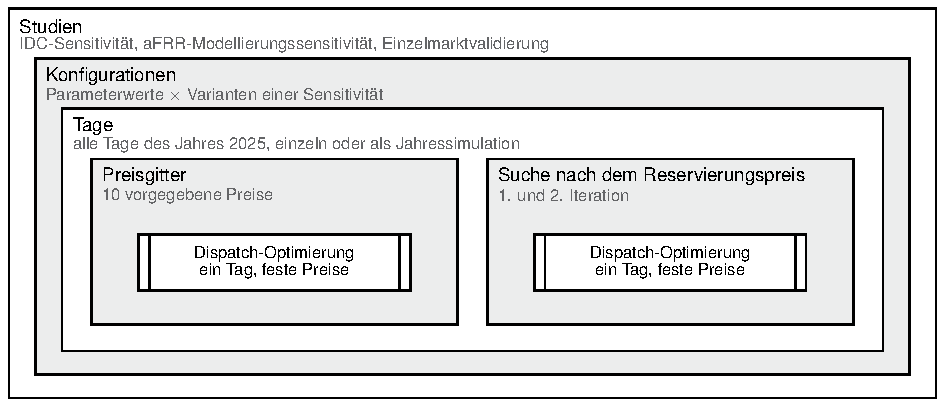
\includegraphics[width=\textwidth]{figures/chapter_3/schleifenebenen.pdf}
    \caption{Schleifen um das Tagesmodell, von der Suche je Tag bis zu Konfigurationen und Studien.}
    \label{fig:schleifenebenen}
\end{figure}

\section{Validierung des Optimierungsmodells}
\label{sec:model_verification}

Die Validierung prüft das Optimierungsmodell in zwei Hinsichten, nämlich die Höhe der Erlöse, die es für ein \ac{BESS} am deutschen Markt ausweist, und seine Funktionsweise, also ob die Optimierung die kurative Reservierung so in den Betrieb einfügt, wie das Produkt es vorsieht.
Für die Erlöshöhe dient der Revenue-Index der Battery Charts als Referenz von außen.
Für die Funktionsweise wird anhand einer Beispieloptimierung nachvollzogen, wie sich die Leistung an einem Beispieltag auf die Märkte verteilt.

\subsection{Vergleichsmaßstab}
\label{sec:validation_benchmark}

Der Revenue-Index der Battery Charts wird vom \ac{ISEA} gemeinsam mit der enspired GmbH entwickelt und weist für ein \ac{BESS} am deutschen Markt den Erlös aus, der mit Regelleistung und Spotmarkthandel erreichbar ist \cite{isea_batterycharts_2026}.
Der Revenue-Index rechnet marktübergreifend, in den Battery Charts \emph{cross-market} genannt, mit der \ac{FCR}, der \ac{aFRR}-Leistung, der \ac{aFRR}-Arbeit und dem kontinuierlichen Intraday-Handel.
Je Markt allein kommen der \ac{DA}, die erste Intraday-Auktion und der \ac{ID1} hinzu \cite{isea_methodik_2026}.
Verwendet ist die Reihe für eine Bezugsanlage mit einem Energieinhalt je Leistung von zwei Stunden, zwei Zyklen je Tag und einem Wirkungsgrad von 95 Prozent je Richtung.
Veröffentlicht wird ein gleitender Mittelwert der Tageserlöse über 365 Tage, sodass der Wert am Jahresende das Kalenderjahr 2025 abbildet.
Die Monatswerte des Vergleichs sind aus diesem Mittelwert zurückgerechnet und treffen ihn für das Jahr 2025 auf ein Prozent.

Marktübergreifend bedient der Revenue-Index die Märkte nacheinander mit fest gesetzten Anteilen an Leistung, Speicherinhalt und Zyklen.
Zuerst wählt der Revenue-Index je Vier-Stunden-Block zwischen der \ac{FCR} und der \ac{aFRR}-Leistung den Markt mit dem höheren Erlös.
Welcher Markt den Block erhält, entscheidet der Revenue-Index anhand der später bekannten Preise beider Märkte.
Die \ac{FCR} bietet 40 Prozent der Leistung an, die \ac{aFRR}-Leistung so viel, wie der Speicher vier Stunden lang liefern könnte, bei der Bezugsanlage also die Hälfte.
Die 40 Prozent ergeben sich, weil der Revenue-Index die Hälfte der Leistung für die \ac{FCR} freihält und die maximale Leistung eines Speichers die angebotene Leistung nach den Präqualifikationsbedingungen um mindestens ein Viertel übersteigen muss \cite{ubertragungsnetzbetreiber_deutschland_praqualifikationsverfahren_2024}.
Der Revenue-Index vergütet in der \ac{FCR} allein die angebotene Leistung und nicht die abgerufene Energie.
Danach bietet der Revenue-Index die \ac{aFRR}-Arbeit zum Preis der ersten Intraday-Auktion mit einem Aufschlag von 50 Prozent an.
Abgerufen wird der Speicher, sobald der Sollwert des \ac{ÜNB} die Leistung aller günstigeren Gebote übersteigt.
Vergütet wird der Abruf zum Grenzpreis der Regelarbeit und nicht zum Gebotspreis.
Geliefert wird der Sollwert, begrenzt auf die vorgehaltene Leistung des Speichers.
Als Daten nutzt der Revenue-Index den sekündlichen Sollwert der deutschen \ac{ÜNB} \cite{netztransparenz_regelenergie_2026} und die anonymisierte Gebotsliste der \ac{aFRR}-Arbeit \cite{regelleistung_ausschreibungsdaten_2026}.
Den Ladezustand hält der Revenue-Index über Geschäfte zum \ac{ID1} im zulässigen Band und führt ihn in den letzten zwei Stunden des Tages auf die Hälfte zurück.
Zuletzt handelt der Revenue-Index im kontinuierlichen Intraday-Handel mit der übrigen Leistung, dem übrigen Speicherinhalt und den übrigen Zyklen, mindestens aber mit der Hälfte der Zyklengrenze, und schließt den Tag mit dem Anfangsladezustand ab.
Als übrige Leistung zieht der Revenue-Index allein die für die \ac{aFRR}-Arbeit vorgehaltene Leistung ab und nicht die Reservierung der \ac{FCR}.
In einem Block mit \ac{FCR}-Zuschlag teilt er deshalb bis zum Anderthalbfachen der Nennleistung zu, nämlich die Hälfte für die \ac{FCR}, ein Viertel für die \ac{aFRR}-Arbeit und drei Viertel für den Intraday-Handel.
Die Aufteilung der Leistung im Revenue-Index taugt damit nicht als Maßstab für die Aufteilung im Optimierungsmodell, während die Höhe des Erlöses als Referenz von außen brauchbar bleibt.

Der kontinuierliche Intraday-Handel läuft rollierend vom Vortag um 16 Uhr bis zum Ende des Liefertages.
Alle 15 Minuten bildet der Revenue-Index aus den Geschäften dieses Zeitfensters je Viertelstundenprodukt den volumengewichteten Preis und optimiert damit ohne Prognose den ganzen Tag neu \cite{semmelmann_algorithm_2024}.
Frühere Geschäfte bleiben bestehen, lassen sich aber glattstellen, sodass der Revenue-Index eine gekaufte Viertelstunde bei gestiegenem Preis zurückverkauft und die Spanne sichert.
Als Preisnehmer handelt der Revenue-Index beliebige Mengen zum volumengewichteten Preis, und Produkte ohne Geschäfte im Zeitfenster bleiben ungehandelt.
Weil ein Handel ohne Marktwirkung den Erlös überschätzt, setzt der Revenue-Index allein den Erlös des Intraday-Handels mit einer Erfassungsrate von 80 Prozent an.

Je Markt allein optimiert der Revenue-Index den Speicher am \ac{DA}, in der ersten Intraday-Auktion und am \ac{ID1} dagegen gegen die bekannte Preisreihe des ganzen Tages.
Gegen die bekannte Preisreihe lädt der Speicher in den günstigsten und entlädt in den teuersten Zeitscheiben, sodass bei zwei Stunden Energieinhalt je Leistung zwei Zyklen die vier günstigsten und die vier teuersten Stunden belegen.
Die Spanne des zweiten Zyklus fällt kleiner aus als die des ersten, weil die Zeitscheiben nach dem Preis geordnet zum Einsatz kommen.

Für das Jahr 2025 weist der Revenue-Index marktübergreifend 259,7 Tausend Euro je Megawatt und Jahr aus.
Je Markt allein erzielt die Bezugsanlage 107,4 Tausend Euro je Megawatt und Jahr in der \ac{FCR}, 221,3 Tausend Euro je Megawatt und Jahr in der \ac{aFRR} mit Leistung und Arbeit, 89,2 Tausend Euro je Megawatt und Jahr am \ac{DA} und 134,1 Tausend Euro je Megawatt und Jahr im kontinuierlichen Intraday-Handel.
Den Werten je Markt allein stehen Jahresläufe des Optimierungsmodells gegenüber, in denen die übrigen Märkte abgeschaltet sind.
Dem marktübergreifenden Wert steht der Referenzerlös aus allen Märkten gegenüber, weil das Optimierungsmodell diese Märkte ebenfalls gemeinsam bedient.
Weil der Revenue-Index keinen \ac{DA} im marktübergreifenden Wert führt, steht ihm dort der Erlös des Optimierungsmodells aus beiden Energiemärkten zusammen gegenüber.

\subsection{Vergleich der Erlöshöhe}
\label{sec:validation_differences}

Revenue-Index und Optimierungsmodell rechnen nach verschiedenen Regeln, sodass vor dem Vergleich die erwartete Abweichung zu klären ist.
Der Revenue-Index bildet erreichbaren Handel ab und erhebt nach eigener Darstellung nicht den Anspruch, den höchsten erzielbaren Erlös zu treffen \cite{isea_methodik_2026}.
Das Optimierungsmodell kennt dagegen alle Preise des Liefertages und setzt jede angebotene Leistung als bezuschlagt.
Die Degradationskosten senken den Erlös des Optimierungsmodells in den Energiemärkten, weil das Optimierungsmodell jeden Zyklus mit Kosten belegt und der Revenue-Index nur eine Zyklengrenze führt.
Der Vergleich soll deshalb allein ausschließen, dass die Modellierung die Erlösmöglichkeiten eines \ac{BESS} unterschätzt.
Der größere Energieinhalt je Leistung des Optimierungsmodells und die fehlende Zyklengrenze wirken in dieselbe Richtung, denn sie erlauben mehr Arbitrage und mehr Vorhaltung je Megawatt.
Erwartet wird, dass das Optimierungsmodell in den Leistungsmärkten über dem Revenue-Index liegt, in den Energiemärkten darunter bleibt und den Jahresgang abbildet.

Der Vergleich beginnt mit den Einzelmärkten, die Anhang~\ref{anh:validierung} im Einzelnen darstellt.
In der \ac{FCR} erreicht das Optimierungsmodell das 1,24-Fache des Revenue-Index, weil der Revenue-Index die angebotene Leistung durch 1,25 teilt und das Optimierungsmodell die volle Leistung anbietet.
Ein Megawatt, das ganzjährig zum \ac{FCR}-Preis anbietet, erzielt 133,0 Tausend Euro je Megawatt und Jahr, wovon der Revenue-Index 81 Prozent und das Optimierungsmodell 100 Prozent erreichen.
In der \ac{aFRR} erreicht das Optimierungsmodell das 1,52-Fache des Revenue-Index, was vor allem an der Bemessung der Leistung liegt.
Der Revenue-Index bietet nur die Leistung an, die der Speicher vier Stunden lang liefern könnte, bei der Bezugsanlage also die Hälfte.
Das Optimierungsmodell ist allein durch ein Ladezustandsband von einer Stunde je Richtung begrenzt und hält im Jahresmittel 81\,\si{MW} in positiver und 72\,\si{MW} in negativer Richtung von 100\,\si{MW} vor.
Auch die Liefermenge der \ac{aFRR}-Arbeit hängt auf beiden Seiten an der vorgehaltenen Leistung, folgt aber verschiedenen Regeln.
Der Revenue-Index liefert nur, wenn sein Gebot im Geld ist, dann aber den realen Abruf bis zu seiner vollen Vorhaltung.
Das Optimierungsmodell liefert dagegen in jeder Viertelstunde mit Abruf einen festen Anteil seiner Vorhaltung, der dem Verhältnis des deutschlandweiten Abrufs zur gesamten Vorhaltung entspricht.
Denselben Sollwert nutzen beide Seiten, der Revenue-Index als abgerufene Leistung und das Optimierungsmodell als Gewicht bei der Mittelung der Grenzpreise.
In den Energiemärkten bleibt das Optimierungsmodell unter dem Revenue-Index, am \ac{DA} mit dem 0,86-Fachen und im Intraday-Handel mit dem 0,89-Fachen.
Die Abweichung folgt den Degradationskosten, die das Optimierungsmodell je Zyklus verrechnet.

\begin{figure}[htbp]
    \centering
    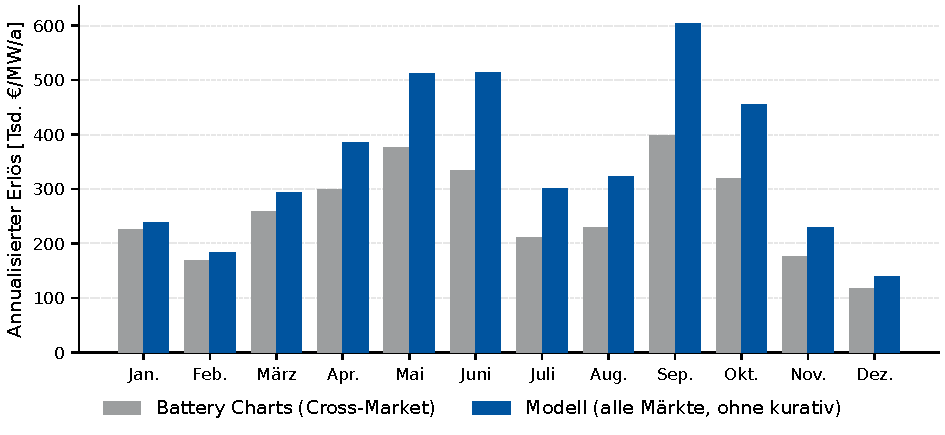
\includegraphics[width=\textwidth]{figures/chapter_3/validierung_cross.pdf}
    \caption{Erlös je Monat 2025 nach Optimierungsmodell und Revenue-Index in Tausend Euro je Megawatt und Jahr, rechts der Abstand beider Reihen.}
    \label{fig:validierung_cross}
\end{figure}

Abbildung~\ref{fig:validierung_cross} stellt marktübergreifend den Revenue-Index dem Referenzerlös des Optimierungsmodells über das Jahr 2025 gegenüber.
Der Revenue-Index liegt im Mittel bei 259,7 Tausend Euro je Megawatt und Jahr, das Optimierungsmodell bei 348,3 Tausend Euro je Megawatt und Jahr.
Das Verhältnis beider Reihen beträgt im Median 1,33 bei einer Spanne von 1,06 bis 1,54, und das Optimierungsmodell liegt in allen zwölf Monaten über dem Revenue-Index.
Die beiden Reihen korrelieren mit einem Koeffizienten von 0,97, sodass das Optimierungsmodell den Jahresgang des Revenue-Index abbildet.
Zum Abstand trägt marktübergreifend die Aufteilung der Leistung bei.
Der Revenue-Index bedient die Märkte in fester Abfolge mit fest gesetzten Anteilen an Leistung, Speicherinhalt und Zyklen, während das Optimierungsmodell alle Märkte gemeinsam optimiert.
Frei entschieden wird im Revenue-Index allein, ob eine Vier-Stunden-Zeitscheibe der \ac{FCR} oder der \ac{aFRR}-Leistung zufällt.
Den größten Abstand tragen dabei die \ac{aFRR}-Märkte, weil das Optimierungsmodell dort mehr Leistung vorhält und deshalb auch mehr Arbeit liefert.
Marktübergreifend zeigt der Vergleich damit keine Unterschätzung der Erlösmöglichkeiten durch die Modellierung.

\subsection{Validierung der Funktionsweise}
\label{sec:validation_function}

Die zweite Prüfung gilt der Funktionsweise, also der Frage, ob die Optimierung die kurative Reservierung so in den Betrieb einfügt, wie das Produkt es vorsieht.
Dafür eignet sich ein Liefertag bei einem festen Reservierungspreis, weil sich dort Fahrplan, Ladezustand und die verdrängten Handelsaktionen unmittelbar ablesen lassen.
Abbildung~\ref{fig:dispatch_festpreis} zeigt den 11.02.2025, den Tag mit dem höchsten Redispatchvolumen des Jahres 2025 \cite{netztransparenz_regelenergie_2026}, bei einem vorgegebenen Reservierungspreis von 5\,\EurMWh{} in beiden Richtungen.
Die Reservierung belegt die Stunden, in denen die übrigen Märkte wenig bieten, in positiver Richtung etwa die Nachtstunden bis vier Uhr und den späten Abend, während die Stunden mit hohem Leistungspreis bei der \ac{aFRR} bleiben und die Vormittags- und Abendstunden dem \ac{DA} und dem \ac{IDC}.
In den reservierten Stunden hält der Ladezustand die Energie oder den Speicherraum für einen Abruf von einer Megawattstunde je Megawatt frei, und Anfang und Ende des Tages liegen bei 125 Megawattstunden.
Der gezeigte Fahrplan enthält die Mindestgröße von 25\,\si{MW} je Zeitscheibe und Richtung, die das Optimierungsmodell gemischt-ganzzahlig macht.
Die Optimierung reserviert damit nur dort, wo der vorgegebene Reservierungspreis die verdrängten Handelsaktionen aufwiegt, und hält die Bänder des Produkts ein, was die Grundlage der Suche nach dem kleinsten vorgegebenen Reservierungspreis bestätigt.
Ohne die Mindestgröße reserviert die Optimierung an diesem Tag in drei Stunden weniger als 25\,\si{MW} Ladeleistung, sodass der kurative Erlös des Tages um 1,4 Prozent höher liegt.
Anhang~\ref{anh:dispatch_ohne} zeigt diesen Fahrplan ohne die Mindestgröße.

\begin{figure}[H]
    \centering
    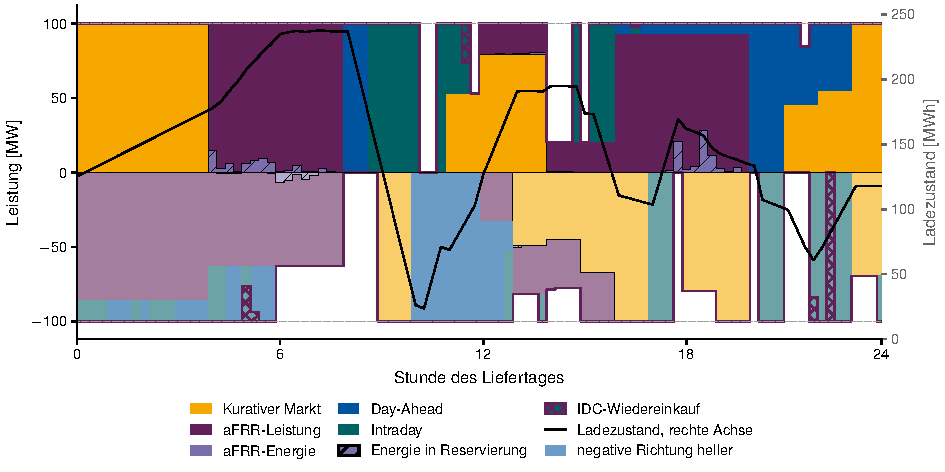
\includegraphics[width=\textwidth]{figures/chapter_3/dispatch_festpreis_2025-02-11_p5.pdf}
    \caption{Fahrplan und Ladezustand am 11.02.2025 bei einem vorgegebenen Reservierungspreis von 5\,\EurMWh{} und der Mindestgröße von 25\,\si{MW}, positive Richtung oben, negative Richtung unten.}
    \label{fig:dispatch_festpreis}
\end{figure}
